%==========================================
%     Documentation for Starry Night above Schuster
%     Compile with pdfLaTeX + BibTeX + pdfLaTeX
%==========================================




\documentclass[a4paper,12pt]{article}

\usepackage{fullpage}
\usepackage{mathtools}
\usepackage{amsmath}
\usepackage{amssymb}
\usepackage{float}
\usepackage{color}
\usepackage{tabularx}
\usepackage{graphicx}
\usepackage[dvipsnames]{xcolor}
\usepackage{caption}
\usepackage{subcaption}
\usepackage{slashed}
\usepackage{booktabs}
\usepackage{pbox}
\usepackage{multirow}
\usepackage{lineno}
\usepackage[a4paper,top=30mm,bottom=25mm,left=21mm,right=21mm, headsep=40pt]{geometry}
\usepackage{braket}
\usepackage{textcomp}
\usepackage{slashed}
\usepackage{bbold}
\usepackage{nicefrac}
\usepackage{arydshln}
\usepackage[style=numeric-comp,sorting=none,backend=bibtex]{biblatex}
\usepackage{enumitem}
\usepackage{fancyhdr}
\usepackage{titlesec}
\usepackage{textcomp}
\usepackage{lscape}
\usepackage{rotating}
\usepackage{setspace}
\usepackage{afterpage}
\usepackage[hidelinks]{hyperref}
\pagestyle{fancy}
\fancyhf{}
\renewcommand{\chaptermark}[1]{\markboth{#1}{}}
\fancyhead[RE]{\textsc{\nouppercase{\leftmark}}}
\fancyhead[lE]{\textsc{\nouppercase{\thepage}}}
\fancyhead[LO]{\textsc{\nouppercase{\leftmark}}}
\fancyhead[RO]{\textsc{\nouppercase{\thepage}}}

%\addtolength{\oddsidemargin}{-12mm}
%\addtolength{\evensidemargin}{-4mm}
%\addtolength{\textwidth}{16mm}
\definecolor{linkcolour}{rgb}{1,0,0}
\hypersetup{colorlinks=true,urlcolor=Blue,linkcolor=Black,anchorcolor=Black,citecolor=Black,filecolor=Black}

\addbibresource{bib/bibliography.bib}

\graphicspath{{figures/}}

\begin{document}

\title{Introduction to limit setting using the $\textit{CL}_{s}$ method}
\author{Stephen Menary, \href{mailto:stmenary@cern.ch}{stmenary@cern.ch}}
\date{Last update: \today}
\maketitle

\begin{abstract}
Limit setting is an important concept within particle physics, especially when the sensitivity of a measurement is expected to be low (e.g. in searches for BSM signatures which might not exist, or SM signals which do not stand out from their respective backgrounds). We introduce the topic of limit setting and contrast the pure-frequentist and $\textit{CL}_s$ methods, the latter of which is widely used by the ATLAS and CMS collaborations. Toy experiments are performed using two simulated BSM-search experiments in order to demonstrate the core-concepts using a minimal working example.
\end{abstract}

\onehalfspace

\section{Introduction} \label{S. Introduction}

Say that we have measured the event yields (/ unfolded cross sections / higher-level observables) in one or many different regions of phase space. We often wish to interpret this result in the context of a particular model, and set limits on certain parameters of this model. Typically we consider limits to be the boundaries of an interval with a high chance of containing the ``true'' parameter value. But what does this really mean? Unfortunately the precise interpretation of a limit is \textit{dependent on the method used}. A Bayesian credible interval is different from a true frequentist interval (``confidence interval''), which is different from a $\textit{CL}_s$ interval. This last point is very important: \textit{a $\textit{CL}_s$ interval is not a true frequentist confidence interval}. However, a $\textit{CL}_s$ interval can be thought of as an approximation to a frequentist interval with one useful extra property. A summary of the three approaches is as follows:

\vspace{0.5cm}
\noindent \textbf{Confidence intervals (frequentist)}
\vspace{0.5cm}

Suppose that our model contains a true parameter, $c_\text{model}$. We have performed an experiment and wish to estimate limits on $c_\text{model}$ based on the results. A confidence interval is \textbf{a set of (one- or two-sided) limits which we expect to contain the ``true'' value of $c_\text{model}$ in a fraction $\alpha$ of all independent experiments}. This means that if $\alpha=95~\%$ then we expect approximately $950$ out of every $1000$ independent experiments to set limits which contain the true value of $c_\text{model}$. This can be stated in a second way: \textbf{any given true $c_\text{model}$ will be excluded by the estimated confidence interval in a fraction $(1-\alpha)$ of experiments}. These are different but equivalent statements.

\newpage
\noindent \textbf{$\textit{CL}_s$ intervals (almost frequentist)}
\vspace{0.5cm}

The $\textit{CL}_s$ method is used to set limits for which the inclusion probability is \textbf{\emph{at least $\alpha$}}. These should not really be called confidence limits in my opinion. There is a good reason for using this method... which we will get to. This benefit comes at the cost of ambiguity, as the inclusion probability is no longer precisely known as it was with frequentist intervals.

\vspace{0.5cm}
\noindent \textbf{Bayesian credible intervals}
\vspace{0.5cm}

Confidence limits are explicitly frequentist as they define probability as the frequency of obtaining a particular result when repeating an experiment. Bayesian statisticians instead define \textit{credible intervals} using the following quantities:
\begin{itemize}
\item $\vec{x}$ represents a possible set of measurements (e.g. event yields in bins of some observable). An individual experiment results in a single measurement $\vec{x}_0$.
\item $P\left( \vec{x}_0 \right)$ is the probability density for obtaining the result $x_0$ out of all possible $\vec{x}$, and is treated as a normalisation constant \cite{Feldman-Cousins-1}.
\item $P\left( c_\text{model} \right)$ is the \textit{prior} probability density distribution on $c_\text{model}$. This represents how much belief we have in $c_\text{model}$ before the experiment. This can have a lot of impact on the result. In principle a non-informative prior on $c_\text{model}$ will result in a credible interval based only on the measured dataset, however a naive uniform prior is not necessarily non-informative because one can always re-parameterise $c_\text{model}\rightarrow c'_\text{model}=f\left(c_\text{model}\right)$ using some nonlinear function $f$ such that a uniform prior on $c_\text{model}$ is equivalent to a non-uniform prior on $c'_\text{model}$. The form of an apprioriate non-informative prior therefore requires consideration of the parameterisation of the model. If e.g. previous measurements have already constrained $c_\text{model}$ then a more restrictive prior can be used.
\item $P\left(\vec{x}_0|c_\text{model}\right)$ is the probability density for obtaining the measurement $\vec{x}_0$ given an assumed value of $c_\text{model}$. We have to construct a model probability density function (PDF) which is valid over the domain of possible measurements, and evaluate it at the measured value $\vec{x}_0$. This is called the \textbf{likelihood function}.
\end{itemize}
Once these quantities have been defined, we can use Bayes' theorem
\begin{equation}
P(A \cup B) = P(A|B) \cdot P(B) = P(B|A) \cdot P(A)
\end{equation}
to infer a \textit{posterior} PDF as a function of $c_\text{model}$ as  
\begin{equation}
P\left(c_\text{model}|\vec{x}_0\right) = \frac{ P\left(\vec{x}_0|c_\text{model}\right) P\left(c_\text{model}\right) }{ P\left(\vec{x}_0\right) } ~~~.
\end{equation}
We can say that we have updated our ``belief'', $P\left(c_\text{model}\right)$, based on the measurement of $\vec{x}_0$. The credible interval is then defined as a set of (one- or two-sided) limits which bound a fraction $\alpha$ of the posterior probability density (normalised to unity over the domain of possible $c_\text{model}$).

We will not consider credible intervals further because they are not often encountered within the context of ATLAS and CMS measurements. Nonetheless, they are important to be aware of as a common statistical tool.


\section{Calculating frequentist limits} \label{S. Calculating limits}

Say that we have some test statistic $q$ which represents the compatibility between a model and the measurement of some observable. Larger values of $q$ mean that the observations become more and more likely under the model hypothesis. Say that we fix the model parameter $c_\text{model}$. Figure~\ref{F. CL from test-stat}(left) then shows a possible expected distribution of $q$. A single experiment is performed, and a value of $q_\text{obs}$ is measured. The \textbf{confidence level (CL)} of this observation is obtained by integrating the expected distribution (normalised to unity) between $-\infty$ and $q_\text{obs}$. This number represents the fraction of experiments which we would expect to produce a result less consistent with the model hypothesis than what was measured, if we assume that particular value of $c_\text{model}$.

\begin{figure}[t!]
\centering
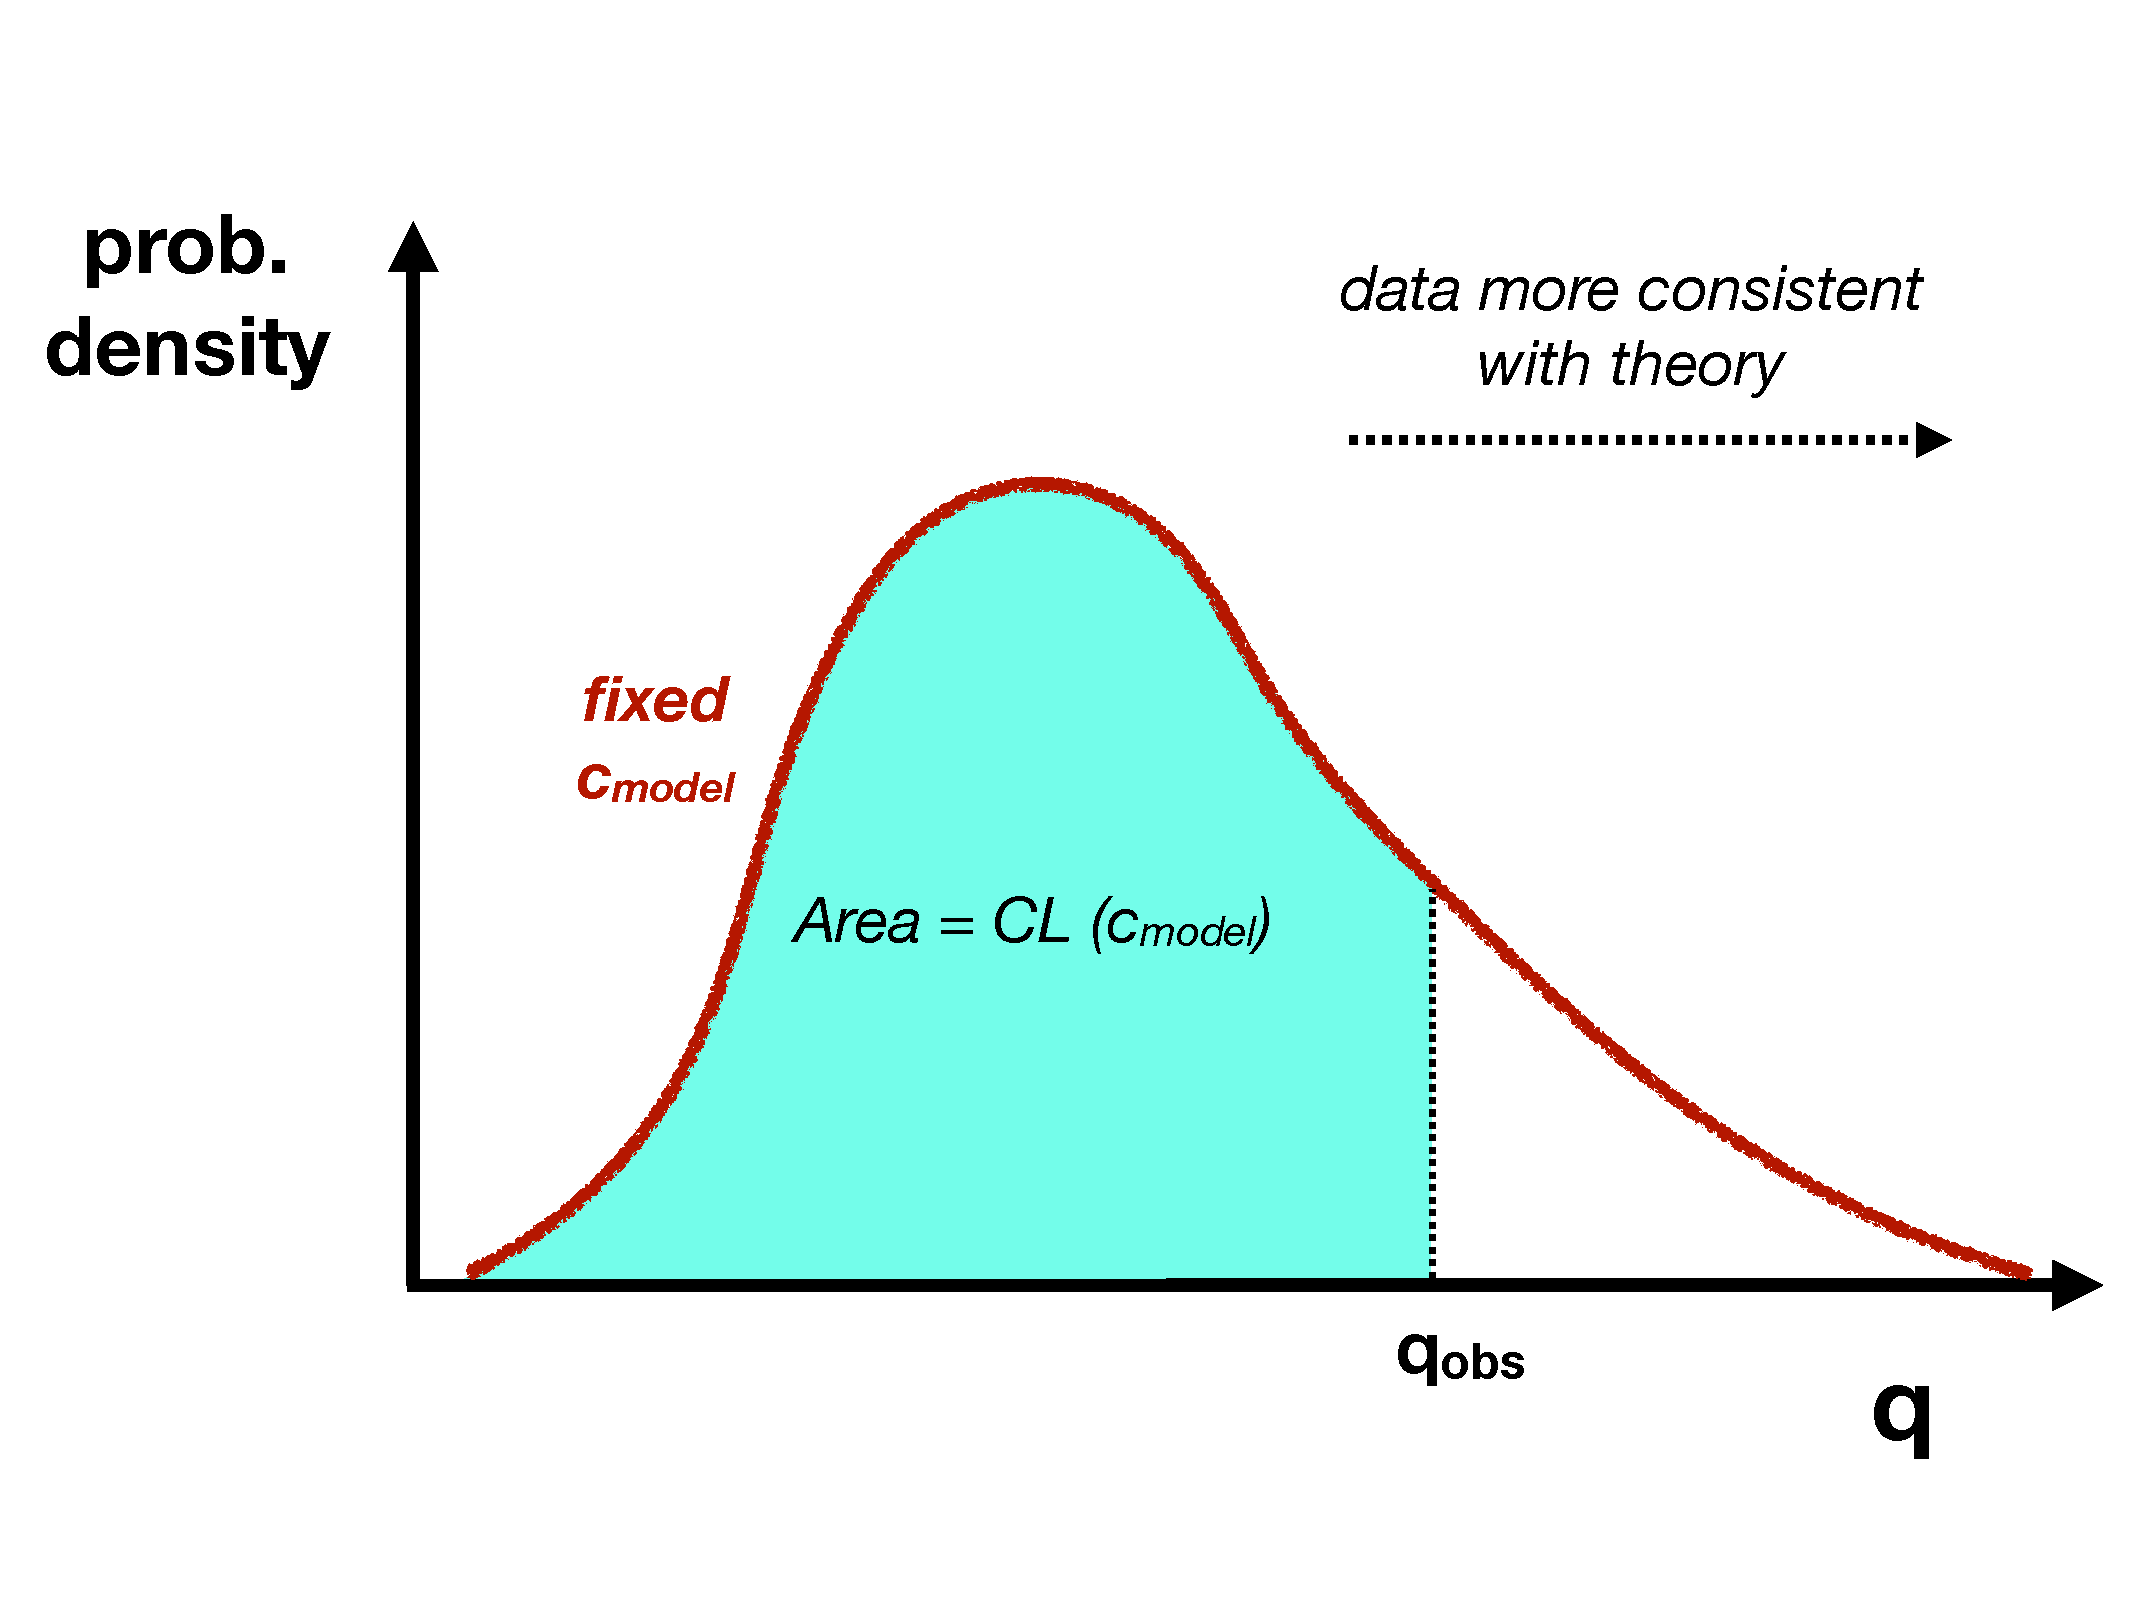
\includegraphics[page=1, width=0.49\textwidth]{TestStatisticDiagram.pdf}
\includegraphics[page=2, width=0.49\textwidth]{TestStatisticDiagram.pdf}
\caption{Left: diagram showing how $\textit{CL}\left(c_\text{model}\right)$ of a single experiment $q_\text{obs}$ is evaluated by integrating over the expected distribution of test statistic $q$ at each scan point in $c_\text{model}$. Right: diagram showing how a frequentist lower-limit on $c_\text{model}$ is extracted from the profile of  $\textit{CL}\left(c_\text{model}\right)$.}
\label{F. CL from test-stat}
\end{figure}

By scanning $c_\text{model}$, we obtain a profile of $\textit{CL}\left(c_\text{model}\right)$ for that experiment. The shape of this profile is dependent on the details of the test statistic measured and the model tested. An example is shown in Figure~\ref{F. CL from test-stat}(right). In this case a lower limit on $c_\text{model}$ is determined by evaluating the region for which $\textit{CL}<1-\alpha$.

\newpage
\noindent \textbf{Likelihood ratio as a test statistic}
\vspace{0.5cm}

The treatment up until now has been very general, not specific to any single model or test statistic. However, a common use-case in particle physics is the search for a signal where there exists an otherwise well-defined null hypothesis (the zero signal case). In this case a common test statistic is the \textbf{likelihood ratio}. The concept of a likelihood was introduced in the previous section. We re-iterate the definition here, now using the special notation $\mathcal{L}$ to denote this important quantity:

 \vspace{0.2cm}
 \begin{table}[h!]
 \begin{tabular}{lc}
\multirow{2}{*}{\textbf{\emph{Likelihood,}} $\mathcal{L}\left(\vec{x}|\vec{\theta}\right)$} \hspace{0.5cm}  & ``the probability density for obtaining a set of measurements  \\
&  $\vec{x}$ \textit{given} a model hypothesis and set of model parameters $\vec\theta$''
\end{tabular}
\end{table}

Note that the likelihood function is a PDF which is normalised over the domain of all possible \textit{measurements} $\vec{x}$, not all possible \textit{parameters} $\vec{\theta}$. This means that the likelihood should indeed be considered as a probabiltiy density, but not over the model parameters. This subtle difference becomes very important when interpreting likelihood profiles later on.

The vector $\vec{\theta}$ can contain so-called \textit{parameters of interest (PoIs)}, i.e. physical quantities which we want to measure or set limits on, and so-called \textit{nuisance parameters (NPs)}, i.e. further quantities which we do not know the true values of and wish to constrain using our data. Nuisance parameters are powerful tools which allow us to account for unknown quantities in our model, and especially for propagating the impact of systematic uncertainties onto the PoIs, however we will not consider this idea for now.

We can construct two models. The null hypothesis is described by a likelihood function of $\mathcal{L}_b\left(\vec{x}|\vec{\theta}_b\right)$. We can perform a \textit{maximum likelihood fit} which varies the NPs contained within $\vec{\theta}_b$ and finds the maximum likelihood $\mathcal{L}^\text{max}_b$. We say that the NPs have been \textit{marginalised}. A particular signal model is described by a likelihood $\mathcal{L}_{s+b}\left(\vec{x}|\vec{\theta}_{s+b}\right)$. In this case we find $\mathcal{L}^\text{max}_{s+b}$ by optimising all relevant PoIs and NPs. The likelihood ratio is defined as 
\begin{equation}
q =
\frac{ \mathcal{L}^\text{max}_{s+b}\left(\vec{x}|\vec{\theta}_{s+b}\right) }{ \mathcal{L}^\text{max}_b\left(\vec{x}|\vec{\theta}_b\right) } ~~~.
\end{equation}
This test statistic is designed to discriminate between measurements consistent with the ``signal plus background'' ($s+b$) and ``background only'' ($b$) hypotheses. It is large when the $s+b$ hypothesis had a significantly larger chance of producing the observed measurement than the $b$ hypothesis.

Note that we \textit{do not} fix $c_\text{model}$ within the fit of $\mathcal{L}^\text{max}_{s+b}\left(\vec{x}|\vec{\theta}_{s+b}\right)$ when evaluating $CL$ for a particular value of $c_\text{model}$. The fit is performed once for the $s+b$ hypothesis with $c_\text{model}$ floating (if even present), and once for the $b$ hypothesis, in order to determine $q_\text{obs}$. This single value is then used to evaluate $CL$ for many possible values of fixed $c_\text{model}$, for which the expected distributions of $q$ were derived in advance. We then evaluate limits using the prescription shown in Figure~\ref{F. CL from test-stat}. This is called the $\textit{CL}_{s+b}$ method. It is important to note that $CL_{s+b}$ results in true frequentist confidence intervals.

% Note that we can control model parameters such as $c_\text{model}$ within $\vec{\theta}_{s+b}$ and evaluate the confidence level at every scan point. 





\section{The $CL_s$ method}
\label{S. CLs}

The \textbf{coverage} of a method is the fraction of experiments for which the true value of a model parameter $c_\text{model}$ lies within the estimated interval. The $CL_{s+b}$ method presented in the previous section defines truly frequentist confidence intervals. This means that the coverage obtained by excluding points for whih $CL_{s+b}\leq\alpha$ is expected to be $\alpha$.

There is one potential drawback of $CL_{s+b}$: the limit set on $c_\text{model}$ may be rather aggressive if there is a large fluctuation in the number of background events. In fact, for two experiments with exactly the same signal rate, the experiment with \textit{more background} may, by chance, set \textit{more stringent limits} than were possible using the experiment with a more modest background rate. This is because statistical fluctuations go as $\sim\sqrt{N}$ where $N=N_\text{sig}+N_\text{bkg}$ is the expected number of events in a bin with $N_\text{sig}$ expected signal events and $N_\text{bkg}$ background. A larger $N_\text{bkg}$ therefore increases $N$, allows for larger downwards fluctuations on the measured event yield, and sets a tighter limit on $N_\text{sig}$. Many people consider this behaviour to be undesirable.

In order to counteract this problem, the $CL_s$ method defines its confidence level as
\begin{equation}
CL_s = \frac{CL_{s+b}}{CL_b}
\end{equation}
where $CL_b$ is the frequentist confidence level evaluated \textit{at the null hypothesis}. Why do we do this? Consider an experiment with an extreme downwards fluctuation. This will not only lead to a small $CL_{s+b}$ but a small $CL_b$. The ratio effectively rescales $CL_{s+b}$ to account for this lowering in $CL_b$. The quantity $CL_s$ is therefore not a true confidence level, but a ratio of confidence levels.

The $CL_s$ method excludes regions for which $CL_s\leq\alpha$. However, this definition \textit{does not} lead to a coverage of $\alpha$. Instead the coverage is $\geq\alpha$. This has to be true because $0\leq CL_b\leq 1$ by definition, and so $\nicefrac{CL_{s+b}}{CL_b}\left(c_\text{model}\right) \geq CL_{s+b}\left(c_\text{model}\right) ~\forall~ c_\text{model}$. The $CL_s$ method does not set truly frequentist limits, but it sets \text{conservative} limits where the coverage is \textit{never less than $\alpha$}. This is often considered an acceptable compromise in order to solve the ``problem'' of inflated exclusion limits from less sensitive experiments.


\section{Toy experiments of $CL_s$ and $CL_{s+b}$}
\label{S. CLs In Action}

We have introduced the $CL_{s+b}$ and $CL_s$ methods and discussed their important properties. Now we implement a simple test-case from which to demonstrate them in practice.


\subsection{Defining the models}
\label{S. CLsInAction::Models}

Say that we measure event yields in bins $i$ of some nameless observable. We have miraculously been able to perform these measurements with no systematic uncertainties. However, they are nonetheless subject to statistical fluctuations around the expected event yields. We have one source of background, which follows a continuous distribution as a function of our observable. We are searching for a bump in this spectrum which we want to interpret as a signal of a dark matter mediator. We claim that we know the background and signal distributions exactly (no systematic uncertainties!), but we do not know anything about their respective rates. The expected event yield in bin $i$ is
\begin{equation}
\nu^\text{exp}_{\text{evt, }i}\left(\mu_\text{sig}, \mu_\text{bkg}\right) = \mu_\text{sig} \cdot \mathcal{S}\left(i\right) + \mu_\text{bkg} \cdot \mathcal{B}\left(i\right)
\label{E. ModelYields}
\end{equation}
where $\mathcal{S}$ is a signal template (known), $\mu_\text{sig}$ is a signal scale factor (unknown),  $\mathcal{B}$ is a background template (known) and $\mu_\text{bkg}$ is its scale factor (unknown). Figure~\ref{F. Asimovs} shows two possible models. Black points are an Asimov dataset, meaning that each measurement has been set to its expected value with an uncertainty reflecting its expected variance. We are performing a counting experiment, so we estimate uncertainties to have a magnitude of $\sqrt{\nu^\text{exp}_{\text{evt, }i}}$ (because we expect them to be Poisson distributed). \texttt{Model 1} has a moderate background rate which allows a non-negligible sensitivity to the signals when $\mu_\text{sig}^\text{true}=1$. \texttt{Model 2} has exactly the same signal and background templates but a signficantly larger background rate.

%This will be used to demonstrate the behaviour used to motivate use of the $CL_s$ method in the previous section.

\begin{figure}[t!]
\centering
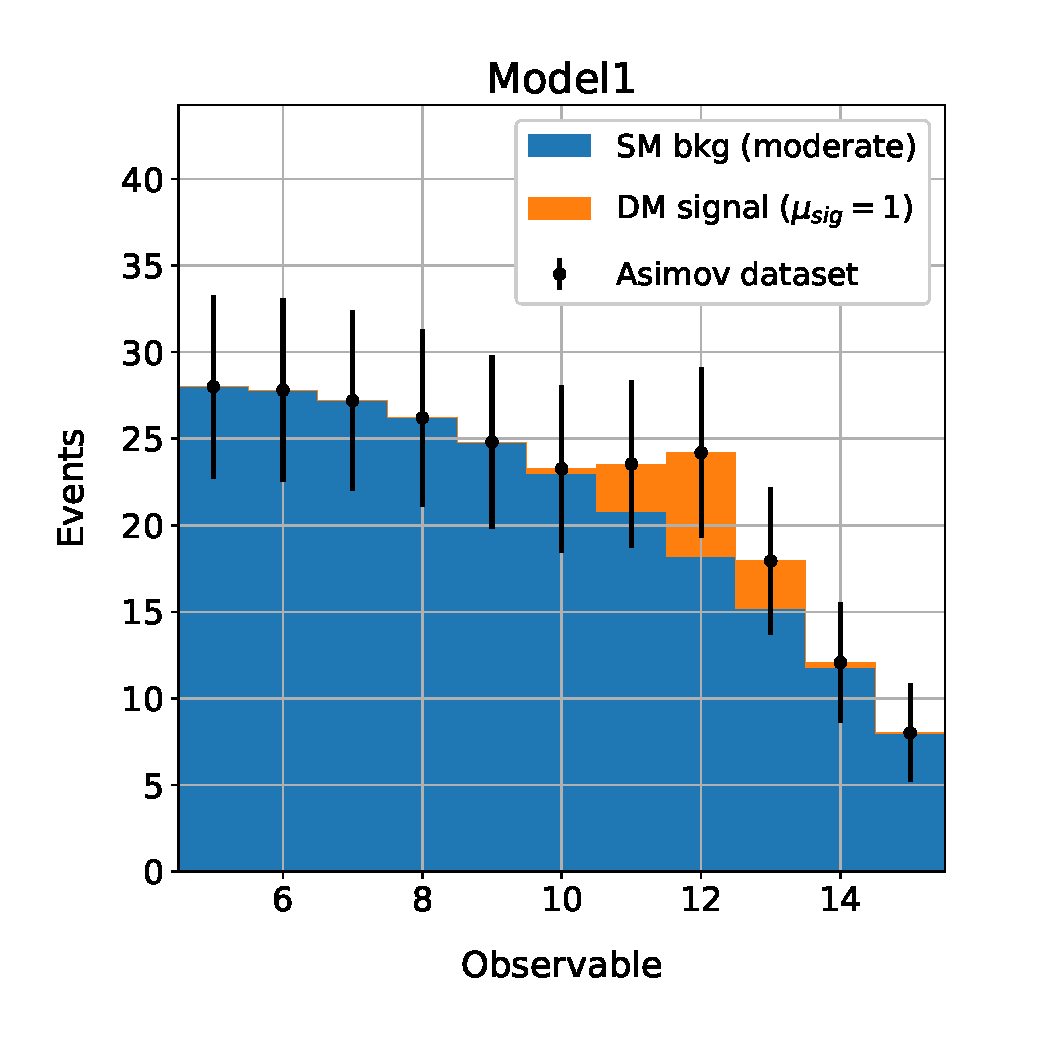
\includegraphics[page=1, width=0.49\textwidth]{ModelDatasets.pdf}
\includegraphics[page=2, width=0.49\textwidth]{ModelDatasets.pdf}
\caption{Left: Asimov dataset for an experiment with $\mu_\text{sig}^\text{true}=1,~\mu_\text{bkg}^\text{true}=0.8$. Right: Asimov dataset for an experiment with $\mu_\text{sig}^\text{true}=1,~\mu_\text{bkg}^\text{true}=5$.}
\label{F. Asimovs}
\end{figure}





\subsection{Defining the likelihood}
\label{S. CLsInAction::Likelihood}

We now define likelihood functions for the $s+b$ and $b$ models. This is easy for event counting experiments without systematic uncertainties. The templates $\mathcal{S}$ and $\mathcal{B}$ are known exactly\footnote{We stress that this is only a result of us not considering systematic uncertainties. In general any lack of model knowledge will be accounted for using NPs.}, perhaps derived in practice using Monte Carlo simulations, but defined here using some arbitrary functions we invented. The expected probability for observing $\nu^\text{obs}_{\text{evt, }i}$ events in bin $i$ follows a Poisson distribution around the expected mean in that bin, $\nu^\text{exp}_{\text{evt, }i}$. Since our bins are statistically independent, the \textit{combined probability} is simply the product of the individual bins. Therefore
\begin{equation}
\begin{aligned}
\mathcal{L}_{s+b} \left(\mu_\text{sig}, \mu_\text{bkg}\right) &=   \text{Poisson}\left( ~ \nu^\text{obs}_{\text{evt, }i}  ~|~  \nu^\text{exp}_{\text{evt, }i} \left(\mu_\text{sig}, \mu_\text{bkg} \right) ~ \right) \\
\mathcal{L}_{b} \left(\mu_\text{bkg}\right) &=   \text{Poisson}\left( ~ \nu^\text{obs}_{\text{evt, }i}  ~|~  \nu^\text{exp}_{\text{evt, }i} \left(0, \mu_\text{bkg} \right) ~ \right) \\
\end{aligned}
\end{equation}
where $\nu^\text{exp}_{\text{evt, }i}$ is defined according to Eq.~\ref{E. ModelYields}. We note an interesting property. In the \textit{asymptotic limit}, which is the limit of infinite event yields (achieved by an experiment with infinite integrated luminosity and $\nu^\text{exp}_{\text{evt, }i}>0 ~\forall~ i$), a Poisson distribution tends towards a Gaussian one. For large datasets, the quantity $-2 \ln \mathcal{L}$ is then expected to follow a $\chi^2$ distribution with degrees of freedom equal to the number of measurements ($N_\text{bins}$). The optimisation process for $-2 \ln \mathcal{L}^\text{max}$ will remove some degrees of freedom. Now, if the $s+b$ and $b$ models are identical but for the inclusion of several \textit{PoIs} in the $s+b$ model, as is true for our model, we find a nice result: $-2 \ln q$ in the asymptotic limit represents a $\Delta \chi^2$ distribution with the number of degrees of freedom equal to the number of PoIs.

For the experiment shown in Figure~\ref{F. Asimovs}, we do not always measure enough events to rely on the asymptotic approximation, and so we will not assume $-2 \ln q$ to be a $\Delta \chi^2$ distribution. However, this fact is too useful not to be mentioned: it will come up very often, and can be used to construct a test statistic $q\sim\exp\left(-\frac{1}{2} \chi^2\right)$ from a set of normally-distributed measurements with known covariance.






\subsection{Bias and coverage of the fit}
\label{S. CLsInAction::BiasCoverage}

An experiment is unbiased if the mean $\langle \vec{\hat{m}} \rangle$ of many repeated estimates $\vec{\hat{m}}$ of some quantity $m$ is equal to its true value $m_\text{true}$. For an unbiased method, Gaussian uncertainty estimates of magnitude $\vec{\hat{\sigma}}$ have the correct coverage if $m_\text{true}$ is contained within the interval bounded by $\hat m_k \pm N\hat\sigma_k$ with the frequency expected by integrating a standard normal distribution over the interval $[-N,N]$, where $k$ labels individual estimates.

We now introduce the concept of a \textbf{pull}. Say that we perform a large number of experiments and calculate
\begin{equation}
\hat p_k = \frac{\hat \mu_k - \mu_\text{ref}}{\hat \sigma_k}
\end{equation}
for each one. We expect that $\hat p$ will be normally distributed around $\left(\mu_\text{true}-\mu_\text{ref}\right)$ provided that our measurement is unbiased and has well estimated Gaussian uncertainties.

We can use this fact to test the bias and coverage of our method. We want to generate an ensemble of estimates and check that the resulting $\vec{\hat{p}}$ have the expected mean and variance. This does not require us to perform our experiment multiple times. Instead we use \textbf{toy datasets} (a.k.a. psuedo-experiments) using the following process.

\begin{figure}[t!]
\centering
\includegraphics[page=3, width=0.49\textwidth]{ModelDatasets.pdf}
\includegraphics[page=4, width=0.49\textwidth]{ModelDatasets.pdf}
\caption{Toy datasets generated for the (left) model 1 and (right) model 2 experiments. Each toy represents a possible statistical fluctuation around the expectation. Toys are generate following the expected Poisson probability distributions. A collection of toys therefore represents a representative sampling of the ensemble of all possible datasets.}
\label{F. Toys}
\end{figure}

In Figure~\ref{F. Asimovs}, we presented an Asimov dataset around the expected model. Instead of setting the datapoints to their expected values, we can instead throw random Poisson fluctuations around these values\footnote{If the expected mean event yield is $N$, then each toy dataset contains a random number of events drawn from a Poisson distribution with mean $N$.}, with uncertainties calculated using these new ``measured'' central values. This creates a toy dataset. Examples are shown in Figure~\ref{F. Toys}. We perform this process many times, creating a collection of statistically independent toys which represent a sampling of the ensemble of all possible datasets.

We perform maximum likelihood fits under the $s+b$ hypothesis to obtain estimates of $\mu_\text{sig}\pm\sigma_\text{sig}$. The PoI uncertainty $\sigma_\text{sig}$ is obtained using either the Hessian matrix or likelihood-scan approach. These will be considered later. We thus obtain the set $\vec{\hat{p}}$. Using $\mu_\text{ref}=\mu_\text{sig}^\text{true}$ we expect
\begin{itemize}
\item The mean of $\vec{\hat{p}}$ is 0 if the method is unbiased.
\item The standard deviation of $\vec{\hat{p}}$ is 1 if the uncertainties have correct coverage.
\end{itemize}

Figure~\ref{F. Pulls} shows the $\vec{\hat{p}}$ distribution obtained under the \texttt{model 1} hypothesis using $\mu_\text{sig}^\text{true}=0$ (left) and $\mu_\text{sig}^\text{true}=3$ (right). Both cases demonstrate good compatibility with the standard normal distributions, which are overlayed for comparison.

\begin{figure}[t!]
\centering
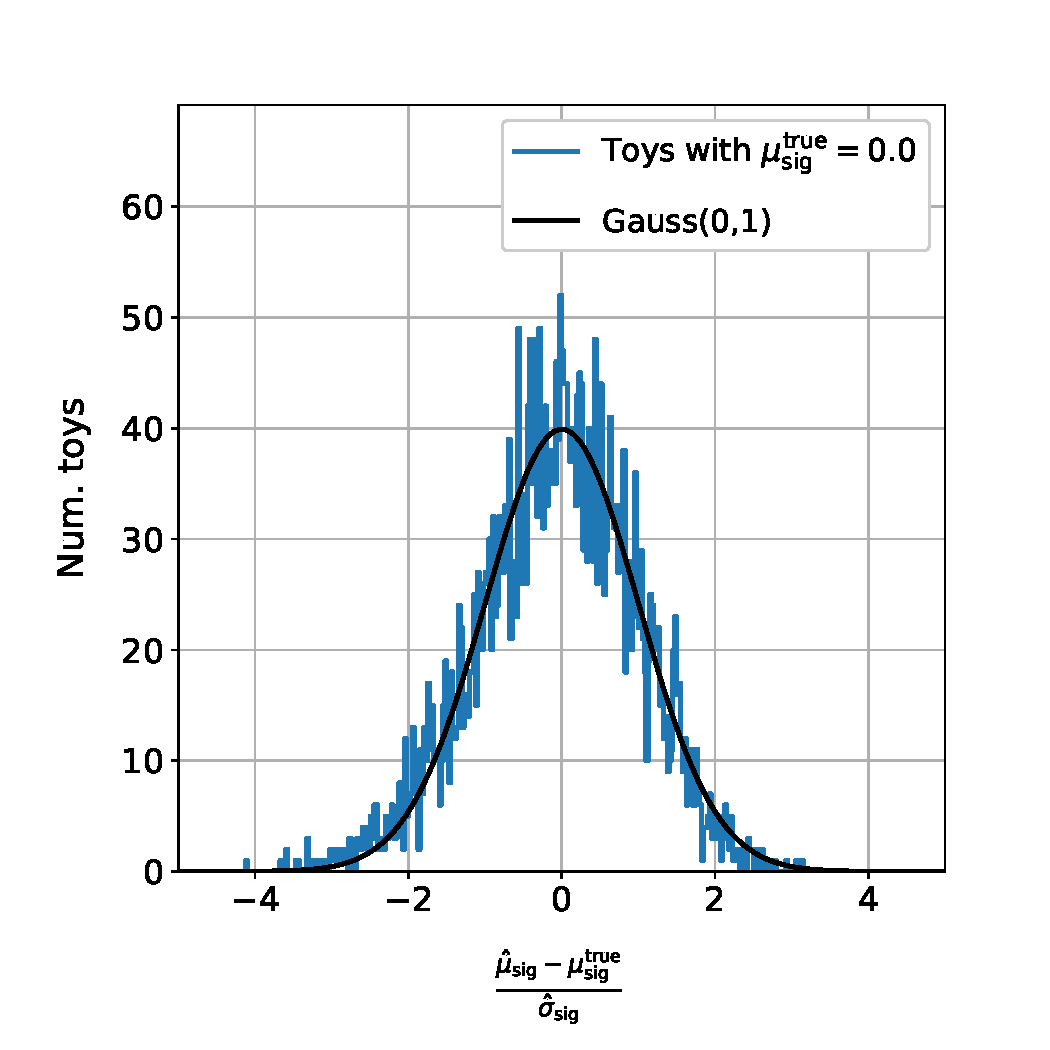
\includegraphics[page=1, width=0.49\textwidth]{Pulls.pdf}
\includegraphics[page=2, width=0.49\textwidth]{Pulls.pdf}
\caption{Distribution of pulls in 4000 toy datasets generated under the model 1 hypothesis with (left) $\mu_\text{sig}^\text{true}=0$ and (right) $\mu_\text{sig}^\text{true}=3$. Standard normal distributions are overlayed for comparison. Good agreement demonstrates a fit procedure with small bias and good coverage.}
\label{F. Pulls}
\end{figure}





\subsection{A note on bias and coverage in the real-world}
\label{S. CLsInAction::BiasCoverage2}

Section~\ref{S. CLsInAction::BiasCoverage} used toy datasets to demonstrate that the fit procedure provided unbiased estimates of the PoI with appropriate uncertainty coverage. This check should always be performed. However, it does not prove that the fit model itself is appropriate in the real-world. For this reason, we should always \textbf{bootstrap} the real-world dataset.

This means that we create psuedo-datasets by varying each datapoint within it's uncertainty\footnote{For an unbinned dataset, we can achieve the desired result by multiplying each datapoint by a Poisson weight with a mean of $1$.} (assuming e.g. Poisson or Gaussian probability densities as appropriate). In this case, we set $\mu_\text{ref}$ equal to the nominal measurement $\mu_\text{sig}^\text{obs}$ around which the fluctuations are applied. Significant deviations of the pull distribution from standard normal indicate that the fit model is not appropriate for the measured dataset. This complements other metrics of compatibility such as goodness-of-fit and NP pull tests.

In summary, the toy tests of Section~\ref{S. CLsInAction::BiasCoverage} should be performed to validate the statistical procedure. The bootstrapping approach of this section should be performed to validate the statistical model.





\subsection{Expected distribution of the test statistic}
\label{S. CLsInAction::TestStatDist}

Generating toy distributions was previously stated to be an effective method for deriving the expected distribution of the PoI pulls accounting for statistical variance. It is also an effective method for deriving the expected distribution of all other quantities. When we generate toys, we are introducing artificial statistical variations according to their expected probability densities, and can thus measure the spread induced on any measurable quantity.

For both the $CL_s$ and $CL_{s+b}$ methods, Figure~\ref{F. CL from test-stat} (left) demonstrated that we must know the expected distribution of the test statistic, $q$, for each possible value of $c_\text{model}=\mu_\text{sig}$. We derive this by generating toy datasets around the model expectation for each scan point in $\mu_\text{sig}$. Two such distributions are shown in Figure~\ref{F. q dist} using the \texttt{model 1} hypothesis under the $b$ hypothesis (left) and a typical scan point (right). When a value $q_\text{obs}$ is measured in a dataset, these distributions allow us to derive $CL_{b}$, $CL_{s+b}$ and thus $CL_s$ for each scan point in $\mu_\text{sig}$.


\begin{figure}[t!]
\centering
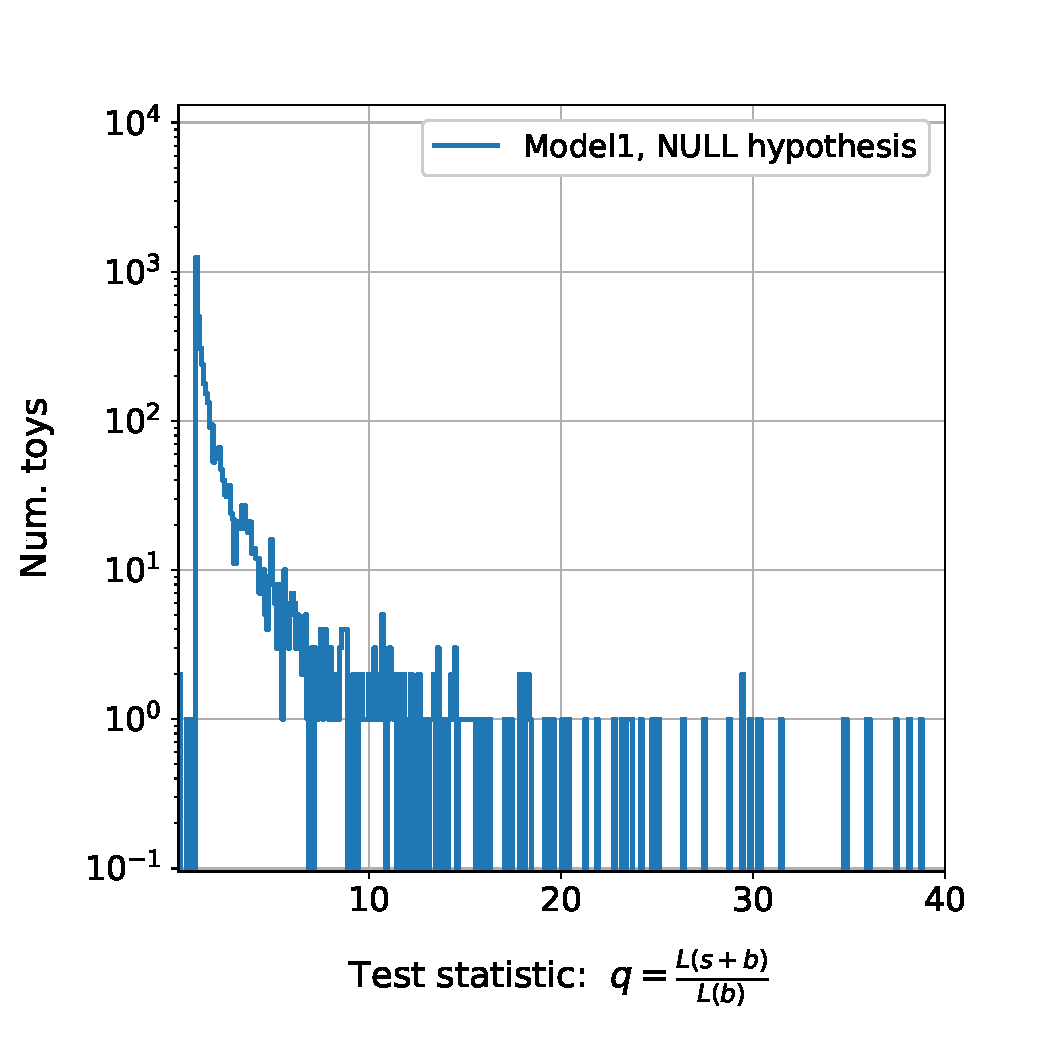
\includegraphics[page=1, width=0.49\textwidth]{TestStatisticToys.pdf}
\includegraphics[page=7, width=0.49\textwidth]{TestStatisticToys.pdf}
\caption{Expected distribution of the test statistic, $q$, evaluated using 4000 toy datasets generated at two different values of $\mu_\text{sig}^\text{true}$.}
\label{F. q dist}
\end{figure}





\subsection{Confidence levels}
\label{S. CLsInAction::ConfidenceLevels}

We are now equipped to evaluate confidence limits. The $CL_{s+b}$ and $CL_s$ profiles are evaluated in all toys. Two examples are shown in Figure~\ref{F. CL curve}. \texttt{Model 1} is used with two different values of $\mu_\text{sig}^\text{true}$. When $\mu_\text{sig}^\text{true}$ is sufficiently large, the $CL_s$ and $CL_{s+b}$ methods provide similar results. This is because all toy datasets are able to exclude the null hypothesis ($b$ only), therefore $\mathcal{L}_b \ll \mathcal{L}_{s+b}$, therefore $q_\text{obs}$ is usually large, therefore $CL_b\approx1~\forall~\mu_\text{sig}$. However, when $\mu_\text{sig}^\text{true}$ is zero, we find $CL_s \geq CL_{s+b}$. In this regime, $CL_s$ limits will be more conservative than the frequentist case.

Based on the shape of the $CL$ profiles in Figure~\ref{F. Coverage}, we can see our measurement will be presented as an upper limit on $\mu_\text{sig}$ if we define limits by excluding the region where $CL\leq95~\%$. We now test the coverage of the two methods. We use the following definition:

 \begin{table}[h!]
 \begin{tabular}{lc}
\multirow{2}{*}{\textbf{\emph{Expected coverage}}} \hspace{0.5cm}  & ``the fraction of toy datasets in which $\mu_\text{sig}^\text{true}$ was excluded with \\
& 95~\% confidence, i.e. for which $CL\left(\mu_\text{sig}=\mu_\text{sig}^\text{true}\right)<0.05$''
\end{tabular}
\end{table}

Using \texttt{model 1}, Figure~\ref{F. Coverage} shows the expected coverage of the $CL_s$ and $CL_{s+b}$ as a function of $\mu_\text{sig}^\text{true}$. Since $CL_{s+b}$ is truly frequentist, we confirm that the expected coverage is always 95~\% by definition. We see that $CL_s$ is conservative for small expected signals and ``overcovers''\footnote{It is not really ``overcovering'' if this is the intended behaviour!} compared with $CL_{s+b}$. As the expected signal increases and unambiguously excludes the null hypothesis, the coverage of $CL_s$ converges towards that of $CL_{s+b}$.

\begin{figure}[!]
\centering
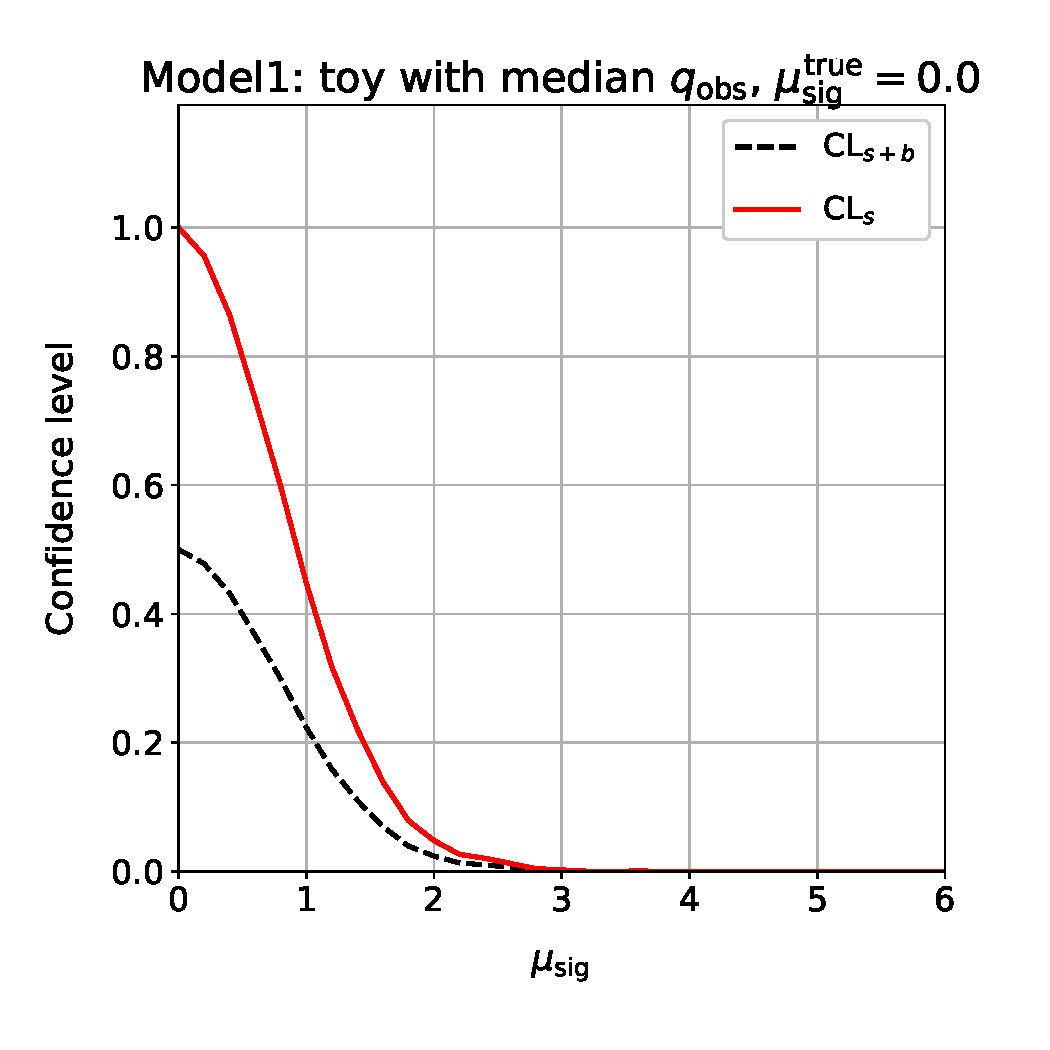
\includegraphics[page=1, width=0.49\textwidth]{CL_and_coverage.pdf}
\includegraphics[page=14, width=0.49\textwidth]{CL_and_coverage.pdf}
\caption{$CL_{s+b}$ and $CL_s$ curves evaluated using individual toys generated under two different $\mu_\text{sig}^\text{true}$ hypotheses using \texttt{model 1}. The toy with median $q_\text{obs}$ is shown.}
\label{F. CL curve}
\vspace{1cm}
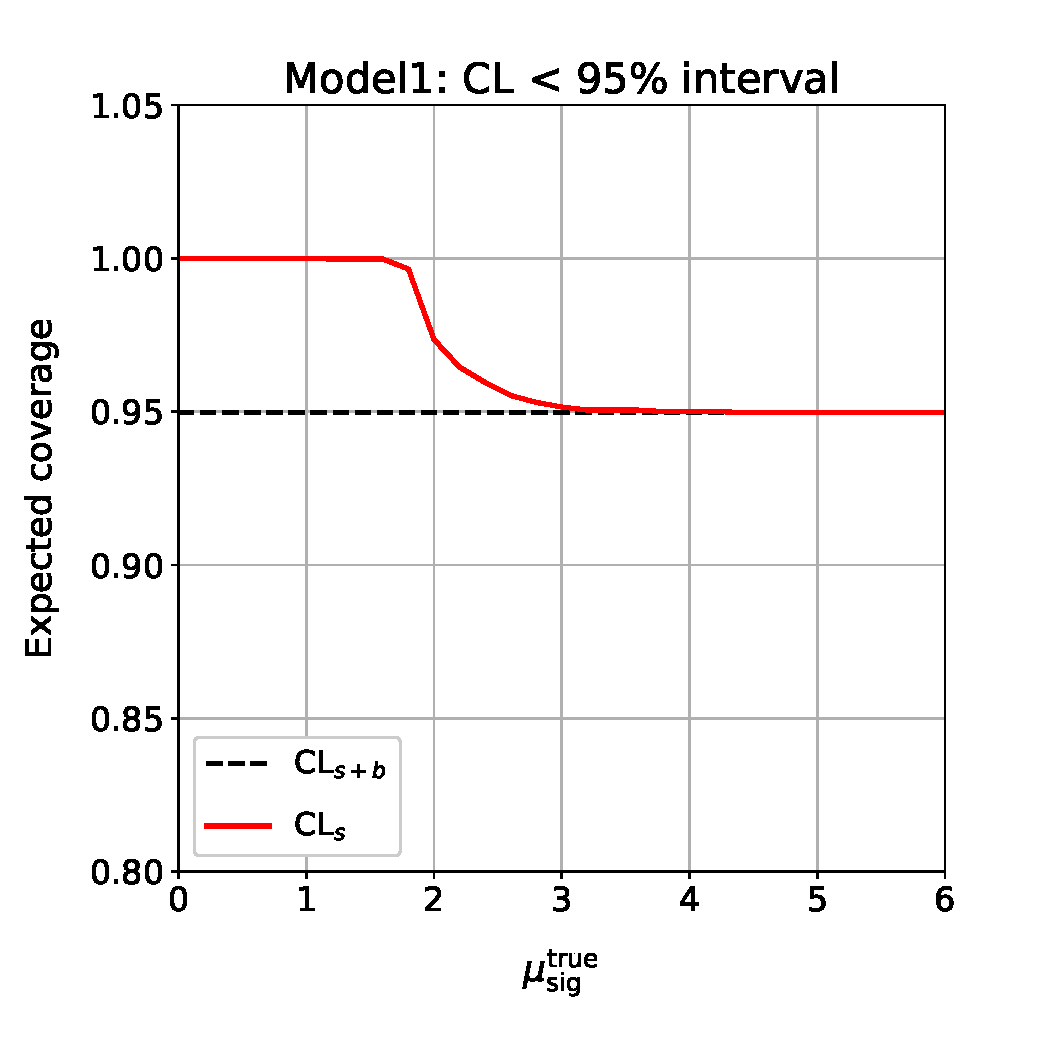
\includegraphics[page=1, width=0.63\textwidth]{Coverage.pdf}
\caption{Coverage of the $CL_{s+b}$ and $CL_s$ methods as a function of $\mu_\text{sig}^\text{true}$ using \texttt{model 1}.}
\label{F. Coverage}
\end{figure}







%\subsection{Summary}
%\label{S. CLsInAction::Summary}
%
%
%- toys --> check stat procedure is unbiased
%- toys --> expected distributions of q
%- toys --> expected coverage (optional)
%- data --> bootstrap to validate fit model
%- data --> 
%



% 


\printbibliography

\clearpage

\end{document}
